\section{Preventivo}
Questa sezione fornisce una stima dei costi che il gruppo dovrà sostenere nelle varie fase\textsubscript{G} che interessano lo svolgimento del progetto\textsubscript{G}. Verranno utilizzate le seguenti abbreviazioni per descrivere l'utilizzo delle risorsa\textsubscript{G} da parte del team:
\begin{itemize}
	\item \textbf{R}: Responsabile
	\item \textbf{V}: Verificatore
	\item \textbf{An}: Analista
	\item \textbf{Am}: Amministratore
	\item \textbf{Pr}: Programmatore
	\item \textbf{Pt}: Progettista
\end{itemize}


\subsection{Avvio}

\subsubsection{Prospetto orario}
Di seguito viene illustrato l'utilizzo della risorsa\textsubscript{G} tempo (espresso in ore) dei vari componenti del gruppo nella fase\textsubscript{G} di Avvio:








\begin{table}[H]
\begin{center}
\begin{tabular}{c
	!{\color[HTML]{9b240a}\vrule width 1pt}
	cccccc
	!{\color[HTML]{9b240a}\vrule width 1pt}	
	c}
\rowcolorhead
\headertitle{Nome} & \headertitle{R} & \headertitle{V} & \headertitle{An} & \headertitle{Am} & \headertitle{Pr} & \headertitle{Pt} & \headertitle{Tot} \\

Chiarello Sofia & 2 & 2 & 5 & 0 & 0 & 0 & 9\\
Crivellari Alberto & 2 & 2 & 5 & 0 & 0 & 0 & 9\\
De Renzis Simone & 4 & 1 & 2 & 3 & 0 & 0 & 10\\
Greggio Nicolò & 2 & 1 & 2 & 5 & 0 & 0 & 10\\
Tessari Andrea & 2 & 2 & 5 & 0 & 0 & 0 & 9\\
Zuccolo Giada & 2 & 2 & 5 & 0 & 0 & 0 & 9\\
\end{tabular}
\caption[Occupazione oraria Avvio]{Per ogni componente, i ruoli ricoperti e la relativa occupazione oraria nella fase\textsubscript{G} di Avvio}
\end{center}
\end{table}


\pgfplotsset{width=10cm,compat=1.17}
\begin{figure}[H]
	\centering
	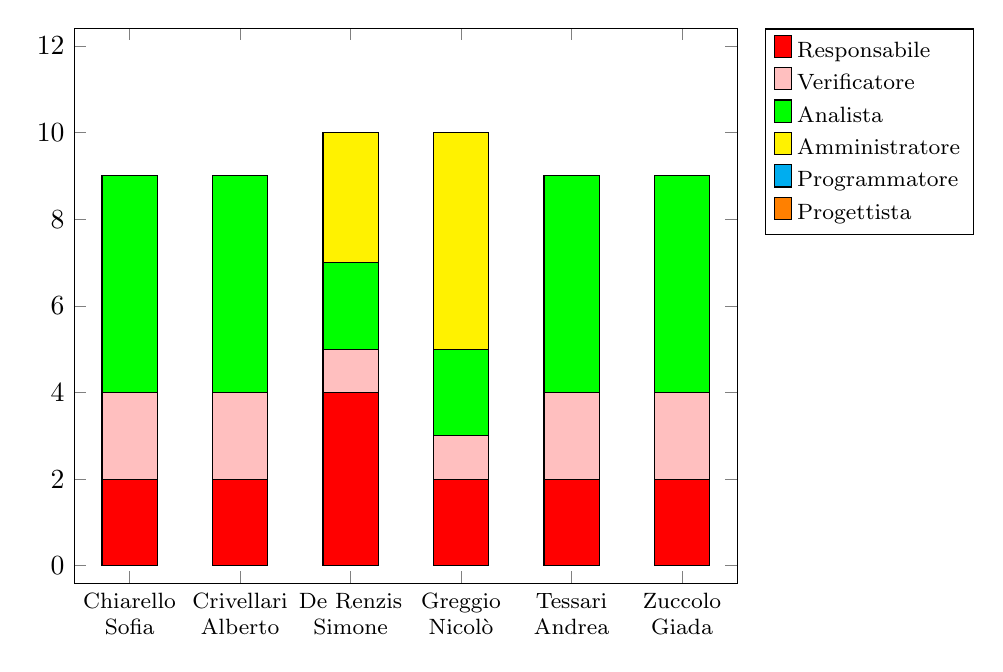
\begin{tikzpicture}
		\begin{axis}[
			enlarge y limits=0.30,
			enlarge x limits=0.10,
			ybar stacked,
			width=10cm,
			bar width=0.7cm,
			%every node near coord/.style={text width=3 cm},
			%nodes near coords,
			%every node near coord/.append style={color=black},
			%enlargelimits=0.25,
			legend style={font=\footnotesize,at={(1.2,1)},
				cells={anchor=west},
				anchor=north,legend columns=1},
			%ylabel={\#participants},
			symbolic x coords={Chiarello Sofia, Crivellari Alberto, De Renzis Simone, Greggio Nicolò, Tessari Andrea, Zuccolo Giada},
			xtick=data,
			x tick label style={font=\footnotesize,text width=1.7cm,align=center},
			]
			\addplot+[ybar,fill=red, draw=black] plot coordinates 
			%Responsabile
				{(Chiarello Sofia,2) 
				(Crivellari Alberto,2) 
				(De Renzis Simone,4) 
				(Greggio Nicolò,2) 
				(Tessari Andrea,2) 
				(Zuccolo Giada,2) };
			\addplot+[ybar,fill=pink, draw=black] plot coordinates 
			%Verificatore
				{(Chiarello Sofia,2) 
				(Crivellari Alberto,2) 
				(De Renzis Simone,1) 
				(Greggio Nicolò,1) 
				(Tessari Andrea,2) 
				(Zuccolo Giada,2) };
			\addplot+[ybar,fill=green, draw=black] plot coordinates 
			%Analista
				{(Chiarello Sofia,5) 
				(Crivellari Alberto,5) 
				(De Renzis Simone,2) 
				(Greggio Nicolò,2) 
				(Tessari Andrea,5) 
				(Zuccolo Giada,5) };
			\addplot+[ybar,fill=yellow, draw=black] plot coordinates
			%Amministratore
				{(Chiarello Sofia,0)
				(Crivellari Alberto,0) 
				(De Renzis Simone,3) 
				(Greggio Nicolò,5)
				(Tessari Andrea,0)
				(Zuccolo Giada,0) };
			\addplot+[ybar,fill=cyan, draw=black] plot coordinates 
			%Programmatore
				{(Chiarello Sofia,0) 
				(Crivellari Alberto,0) 
				(De Renzis Simone,0) 
				(Greggio Nicolò,0) 
				(Tessari Andrea,0) 
				(Zuccolo Giada,0) };
			\addplot+[ybar,fill=orange, draw=black] plot coordinates
			%Progettista
				{(Chiarello Sofia,0) 
				(Crivellari Alberto,0) 
				(De Renzis Simone,0)
				(Greggio Nicolò,0) 
				(Tessari Andrea,0) 
				(Zuccolo Giada,0) };
			\legend{Responsabile \\ Verificatore \\ Analista \\ Amministratore \\ Programmatore \\ Progettista \\}
		\end{axis}
	\end{tikzpicture}
	\caption[Istogramma distribuzione oraria Avvio]{Istogramma che visualizza la ripartizione delle ore nella fase\textsubscript{G} di Avvio} 
\end{figure}






\subsubsection{Prospetto economico}
Il costo derivante dalle ore impiegate dai componenti nella fase\textsubscript{G} di Avvio è descritto di seguito, calcolandone il totale.

\begin{table}[H]
{\setlength{\parindent}{0cm}
\begin{minipage}{.43\textwidth}
	\begin{tabular}{ccc}
	\rowcolorhead
	\headertitle{Ruolo} & \headertitle{Ore} & \headertitle{Costo(\euro{})}\\
	Responsabile & 14 & 420\\
	Verificatore & 10 & 150\\
	Analista & 24 & 600\\
	Amministratore & 8 & 160\\
	Programmatore & 0 & 0\\
	Progettista & 0 & 0\\
	\hline
	\textbf{Totale} & \textbf{56} & \textbf{1330}\\
	\end{tabular}
\end{minipage}% This must go next to `\end{minipage}`
\begin{minipage}{.57\textwidth}
  \begin{tikzpicture}
\pie [rotate = 180,
    sum = auto,
    before number=\pgfsetfillopacity{0.0},
    %text = legend, 
    radius = 2.7,
    color = {red, pink, green, yellow}]
    {    
    150/Verificatore,    
    160/Amministratore,
    420/Responsabile,
    600/Analista
    }
\end{tikzpicture} 
\end{minipage} }
\caption[Prospetto economico della fase\textsubscript{G} di Avvio]{Per ogni ruolo, il complessivo delle ore impiegate dai membri e il relativo ammontare in denaro. Il diagramma a torta visualizza la composizione dei costi nella fase\textsubscript{G} di Avvio}
\end{table}



\subsection{Analisi dei Requisiti}

\subsubsection{Prospetto orario}
Di seguito viene illustrato l'utilizzo della risorsa\textsubscript{G} tempo (espresso in ore) dei vari componenti del gruppo nella fase\textsubscript{G} di Analisi dei Requisiti:

\begin{table}[H]
	\begin{center}
		\begin{tabular}{c
				!{\color[HTML]{9b240a}\vrule width 1pt}
				cccccc
				!{\color[HTML]{9b240a}\vrule width 1pt}	
				c}
			\rowcolorhead
			\headertitle{Nome} & \headertitle{R} & \headertitle{V} & \headertitle{An} & \headertitle{Am} & \headertitle{Pr} & \headertitle{Pt} & \headertitle{Tot} \\
			
			Chiarello Sofia & 0 & 6 & 18 & 1 & 0 & 0 & 25\\
			Crivellari Alberto & 0 & 18 & 4 & 2 & 0 & 0 & 24\\
			De Renzis Simone & 12 & 5 & 5 & 3 & 0 & 0 & 25\\
			Greggio Nicolò & 5 & 5 & 5 & 12 & 0 & 0 & 27\\
			Tessari Andrea & 8 & 5 & 4 & 8 & 0 & 0 & 25\\
			Zuccolo Giada & 0 & 6 & 18 & 1 & 0 & 0 & 25\\
		\end{tabular}
		\caption[Occupazione oraria Analisi dei Requisiti]{Per ogni componente, i ruoli ricoperti e la relativa occupazione oraria nella fase\textsubscript{G} di Analisi dei Requisiti}
	\end{center}
\end{table}


\pgfplotsset{width=10cm,compat=1.17}
\begin{figure}[H]
	\centering
	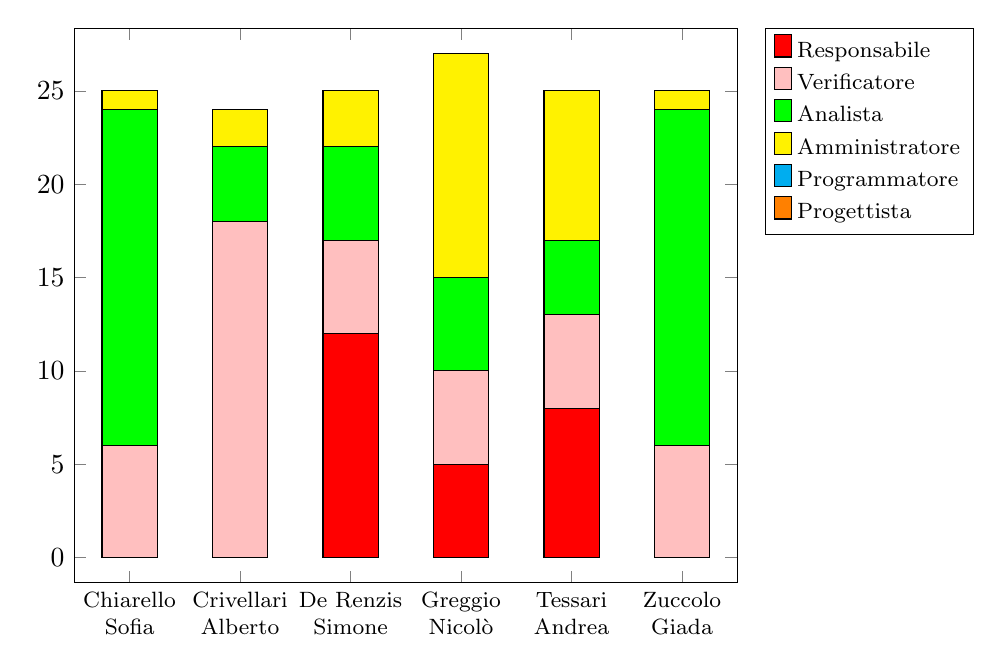
\begin{tikzpicture}
		\begin{axis}[
			enlarge y limits=0.05,
			enlarge x limits=0.10,
			ybar stacked,
			width=10cm,
			bar width=0.7cm,
			%every node near coord/.style={text width=3 cm},
			%nodes near coords,
			%every node near coord/.append style={color=black},
			%enlargelimits=0.25,
			legend style={font=\footnotesize,at={(1.2,1)},
				cells={anchor=west},
				anchor=north,legend columns=1},
			%ylabel={\#participants},
			symbolic x coords={Chiarello Sofia, Crivellari Alberto, De Renzis Simone, Greggio Nicolò, Tessari Andrea, Zuccolo Giada},
			xtick=data,
			x tick label style={font=\footnotesize,text width=1.7cm,align=center},
			]
			\addplot+[ybar,fill=red, draw=black] plot coordinates 
			%Responsabile
			{(Chiarello Sofia,0) 
				(Crivellari Alberto,0) 
				(De Renzis Simone,12) 
				(Greggio Nicolò,5) 
				(Tessari Andrea,8) 
				(Zuccolo Giada,0) };
			\addplot+[ybar,fill=pink, draw=black] plot coordinates 
			%Verificatore
			{(Chiarello Sofia,6) 
				(Crivellari Alberto,18) 
				(De Renzis Simone,5) 
				(Greggio Nicolò,5) 
				(Tessari Andrea,5) 
				(Zuccolo Giada,6) };
			\addplot+[ybar,fill=green, draw=black] plot coordinates 
			%Analista
			{(Chiarello Sofia,18) 
				(Crivellari Alberto,4) 
				(De Renzis Simone,5) 
				(Greggio Nicolò,5) 
				(Tessari Andrea,4) 
				(Zuccolo Giada,18) };
			\addplot+[ybar,fill=yellow, draw=black] plot coordinates
			%Amministratore
			{(Chiarello Sofia,1)
				(Crivellari Alberto,2) 
				(De Renzis Simone,3) 
				(Greggio Nicolò,12)
				(Tessari Andrea,8)
				(Zuccolo Giada,1) };
			\addplot+[ybar,fill=cyan, draw=black] plot coordinates 
			%Programmatore
			{(Chiarello Sofia,0) 
				(Crivellari Alberto,0) 
				(De Renzis Simone,0) 
				(Greggio Nicolò,0) 
				(Tessari Andrea,0) 
				(Zuccolo Giada,0) };
			\addplot+[ybar,fill=orange, draw=black] plot coordinates
			%Progettista
			{(Chiarello Sofia,0) 
				(Crivellari Alberto,0) 
				(De Renzis Simone,0)
				(Greggio Nicolò,0) 
				(Tessari Andrea,0) 
				(Zuccolo Giada,0) };
			\legend{Responsabile \\ Verificatore \\ Analista \\ Amministratore \\ Programmatore \\ Progettista \\}
		\end{axis}
	\end{tikzpicture}
	\caption[Istogramma distribuzione oraria Analisi dei Requisiti]{Istogramma che visualizza la ripartizione delle ore nella fase\textsubscript{G} di Analisi dei Requisiti} 
\end{figure}


\subsubsection{Prospetto economico}
Il costo derivante dalle ore impiegate dai componenti nella fase\textsubscript{G} di Analisi dei Requisiti è descritto di seguito, calcolandone il totale.

\begin{table}[H]
	{\setlength{\parindent}{0cm}
		\begin{minipage}{.43\textwidth}
			\begin{tabular}{ccc}
				\rowcolorhead
				\headertitle{Ruolo} & \headertitle{Ore} & \headertitle{Costo(\euro{})}\\
				Responsabile & 25 & 750\\
				Verificatore & 45 & 675\\
				Analista & 54 & 1350\\
				Amministratore & 27 & 540\\
				Programmatore & 0 & 0\\
				Progettista & 0 & 0\\
				\hline
				\textbf{Totale} & \textbf{151} & \textbf{3315}\\
			\end{tabular}
		\end{minipage}% This must go next to `\end{minipage}`
		\begin{minipage}{.57\textwidth}
			\begin{tikzpicture}
				\pie [rotate = 180,
				sum = auto, 
				before number=\pgfsetfillopacity{0.0},
				%text = legend, 
				radius = 2.7,
				color = {red, pink, green, yellow}]
				{    
					540/Verificatore,    
					675/Amministratore,
					750/Responsabile,
					1350/Analista
				}
			\end{tikzpicture} 
	\end{minipage} }
	\caption[Prospetto economico della fase\textsubscript{G} di Analisi dei Requisiti]{Per ogni ruolo, il complessivo delle ore impiegate dai membri e il relativo ammontare in denaro. Il diagramma a torta visualizza la composizione dei costi nella fase\textsubscript{G} di Analisi dei Requisiti}
\end{table}




\subsection{Progettazione Architetturale}

\subsubsection{Prospetto orario}
Di seguito viene illustrato l'utilizzo della risorsa\textsubscript{G} tempo (espresso in ore) dei vari componenti del gruppo nella fase\textsubscript{G} di Progettazione Architetturale:

\begin{table}[H]
	\begin{center}
		\begin{tabular}{c
				!{\color[HTML]{9b240a}\vrule width 1pt}
				cccccc
				!{\color[HTML]{9b240a}\vrule width 1pt}	
				c}
			\rowcolorhead
			\headertitle{Nome} & \headertitle{R} & \headertitle{V} & \headertitle{An} & \headertitle{Am} & \headertitle{Pr} & \headertitle{Pt} & \headertitle{Tot} \\
			
			Chiarello Sofia & 1 & 2 & 4 & 0 & 8 & 15 & 30\\
			Crivellari Alberto & 1 & 6 & 0 & 0 & 20 & 3 & 30\\
			De Renzis Simone & 4 & 2 & 0 & 2 & 7 & 14 & 29\\
			Greggio Nicolò & 1 & 2 & 0 & 5 & 7 & 13 & 28\\
			Tessari Andrea & 2 & 2 & 0 & 4 & 20 & 2 & 30\\
			Zuccolo Giada & 1 & 2 & 4 & 0 & 8 & 15 & 30\\
		\end{tabular}
		\caption[Occupazione oraria Progettazione Architetturale]{Per ogni componente, i ruoli ricoperti e la relativa occupazione oraria nella fase\textsubscript{G} di Progettazione Architetturale}
	\end{center}
\end{table}


\pgfplotsset{width=10cm,compat=1.17}
\begin{figure}[H]
	\centering
	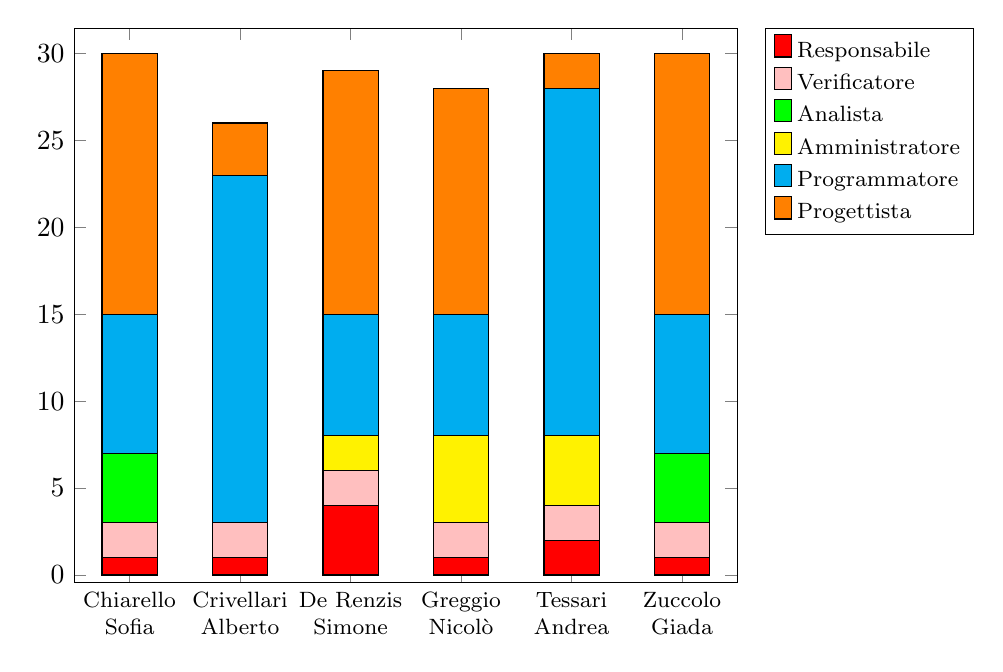
\begin{tikzpicture}
		\begin{axis}[
			enlarge y limits=0.05,
			enlarge x limits=0.10,
			ybar stacked,
			width=10cm,
			bar width=0.7cm,
			%every node near coord/.style={text width=3 cm},
			%nodes near coords,
			%every node near coord/.append style={color=black},
			%enlargelimits=0.25,
			legend style={font=\footnotesize,at={(1.2,1)},
				cells={anchor=west},
				anchor=north,legend columns=1},
			%ylabel={\#participants},
			symbolic x coords={Chiarello Sofia, Crivellari Alberto, De Renzis Simone, Greggio Nicolò, Tessari Andrea, Zuccolo Giada},
			xtick=data,
			x tick label style={font=\footnotesize,text width=1.7cm,align=center},
			]
			\addplot+[ybar,fill=red, draw=black] plot coordinates 
			%Responsabile
			{(Chiarello Sofia,1) 
				(Crivellari Alberto,1) 
				(De Renzis Simone,4) 
				(Greggio Nicolò,1) 
				(Tessari Andrea,2) 
				(Zuccolo Giada,1) };
			\addplot+[ybar,fill=pink, draw=black] plot coordinates 
			%Verificatore
			{(Chiarello Sofia,2) 
				(Crivellari Alberto,2) 
				(De Renzis Simone,2) 
				(Greggio Nicolò,2) 
				(Tessari Andrea,2) 
				(Zuccolo Giada,2) };
			\addplot+[ybar,fill=green, draw=black] plot coordinates 
			%Analista
			{(Chiarello Sofia,4) 
				(Crivellari Alberto,0) 
				(De Renzis Simone,0) 
				(Greggio Nicolò,0) 
				(Tessari Andrea,0) 
				(Zuccolo Giada,4) };
			\addplot+[ybar,fill=yellow, draw=black] plot coordinates
			%Amministratore
			{(Chiarello Sofia,0)
				(Crivellari Alberto,0) 
				(De Renzis Simone,2) 
				(Greggio Nicolò,5)
				(Tessari Andrea,4)
				(Zuccolo Giada,0) };
			\addplot+[ybar,fill=cyan, draw=black] plot coordinates 
			%Programmatore
			{(Chiarello Sofia,8) 
				(Crivellari Alberto,20) 
				(De Renzis Simone,7) 
				(Greggio Nicolò,7) 
				(Tessari Andrea,20) 
				(Zuccolo Giada,8) };
			\addplot+[ybar,fill=orange, draw=black] plot coordinates
			%Progettista
			{(Chiarello Sofia,15) 
				(Crivellari Alberto,3) 
				(De Renzis Simone,14)
				(Greggio Nicolò,13) 
				(Tessari Andrea,2) 
				(Zuccolo Giada,15) };
			\legend{Responsabile \\ Verificatore \\ Analista \\ Amministratore \\ Programmatore \\ Progettista \\}
		\end{axis}
	\end{tikzpicture}
	\caption[Istogramma distribuzione oraria Progettazione Architetturale]{Istogramma che visualizza la ripartizione delle ore nella fase\textsubscript{G} di Progettazione Architetturale} 
\end{figure}


\subsubsection{Prospetto economico}
Il costo derivante dalle ore impiegate dai componenti nella fase\textsubscript{G} di Progettazione Architetturale è descritto di seguito, calcolandone il totale.

\begin{table}[H]
	{\setlength{\parindent}{0cm}
		\begin{minipage}{.43\textwidth}
			\begin{tabular}{ccc}
				\rowcolorhead
				\headertitle{Ruolo} & \headertitle{Ore} & \headertitle{Costo(\euro{})}\\
				Responsabile & 10 & 300\\
				Verificatore & 16 & 240\\
				Analista & 8 & 200\\
				Amministratore & 11 & 220\\
				Programmatore & 70 & 1050\\
				Progettista & 62 & 1364\\
				\hline
				\textbf{Totale} & \textbf{177} & \textbf{3374}\\
			\end{tabular}
		\end{minipage}% This must go next to `\end{minipage}`
		\begin{minipage}{.57\textwidth}
		\begin{tikzpicture}
			\pie [rotate = 270,
			sum = auto, 
			before number=\pgfsetfillopacity{0.0},
			%text = legend, 
			radius = 2.7,
			color = {red, pink, green, yellow, cyan, orange}]
			{
				300/Responsabile,
				240/Verificatore,
				200/Analista,
				220/Amministratore,
				1050/Programmatore,
				1364/Progettista
			}
		\end{tikzpicture} 
	\end{minipage} }
	\caption[Prospetto economico della fase\textsubscript{G} di Analisi dei Requisiti]{Per ogni ruolo, il complessivo delle ore impiegate dai membri e il relativo ammontare in denaro. Il diagramma a torta visualizza la composizione dei costi nella fase\textsubscript{G} di Analisi dei Requisiti}
\end{table}







\subsection{Progettazione di Dettaglio e Codifica dei Requisiti Obbligatori}



\subsubsection{Prospetto orario}
Di seguito viene illustrato l'utilizzo della risorsa\textsubscript{G} tempo (espresso in ore) dei vari componenti del gruppo nella fase\textsubscript{G} di Progettazione e Codifica dei Requisiti Obbligatori:

\begin{table}[H]
	\begin{center}
		\begin{tabular}{c
				!{\color[HTML]{9b240a}\vrule width 1pt}
				cccccc
				!{\color[HTML]{9b240a}\vrule width 1pt}	
				c}
			\rowcolorhead
			\headertitle{Nome} & \headertitle{R} & \headertitle{V} & \headertitle{An} & \headertitle{Am} & \headertitle{Pr} & \headertitle{Pt} & \headertitle{Tot} \\
			
			Chiarello Sofia & 0 & 15 & 2 & 0 & 22 & 6 & 45\\
			Crivellari Alberto & 0 & 20 & 0 & 1 & 5 & 20 & 46\\
			De Renzis Simone & 2 & 14 & 0 & 0 & 21 & 8 & 45\\
			Greggio Nicolò & 1 & 14 & 0 & 3 & 21 & 5 & 44\\
			Tessari Andrea & 1 & 15 & 0 & 0 & 5 & 25 & 46\\
			Zuccolo Giada & 0 & 14 & 2 & 2 & 23 & 4 & 45\\
		\end{tabular}
		\caption[Occupazione oraria Progettazione e Codifica dei Requisiti Obbligatori]{Per ogni componente, i ruoli ricoperti e la relativa occupazione oraria nella fase\textsubscript{G} di Progettazione e Codifica dei Requisiti Obbligatori}
	\end{center}
\end{table}


\pgfplotsset{width=10cm,compat=1.17}
\begin{figure}[H]
	\centering
	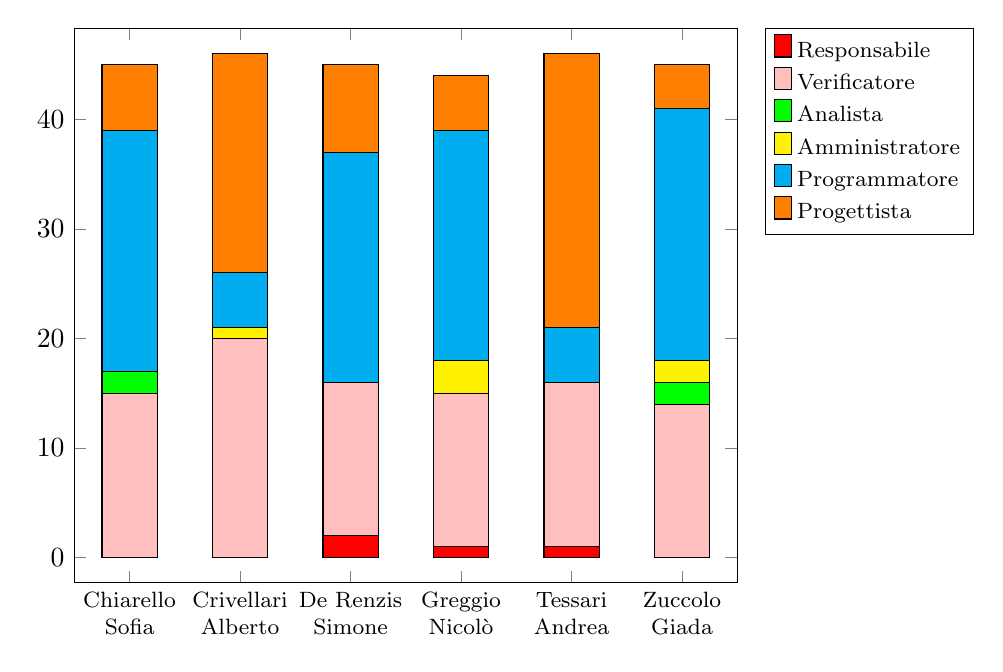
\begin{tikzpicture}
		\begin{axis}[
			enlarge y limits=0.05,
			enlarge x limits=0.10,
			ybar stacked,
			width=10cm,
			bar width=0.7cm,
			%every node near coord/.style={text width=3 cm},
			%nodes near coords,
			%every node near coord/.append style={color=black},
			%enlargelimits=0.25,
			legend style={font=\footnotesize,at={(1.2,1)},
				cells={anchor=west},
				anchor=north,legend columns=1},
			%ylabel={\#participants},
			symbolic x coords={Chiarello Sofia, Crivellari Alberto, De Renzis Simone, Greggio Nicolò, Tessari Andrea, Zuccolo Giada},
			xtick=data,
			x tick label style={font=\footnotesize,text width=1.7cm,align=center},
			]
			\addplot+[ybar,fill=red, draw=black] plot coordinates 
			%Responsabile
			{(Chiarello Sofia,0) 
				(Crivellari Alberto,0) 
				(De Renzis Simone,2) 
				(Greggio Nicolò,1) 
				(Tessari Andrea,1) 
				(Zuccolo Giada,0) };
			\addplot+[ybar,fill=pink, draw=black] plot coordinates 
			%Verificatore
			{(Chiarello Sofia,15) 
				(Crivellari Alberto,20) 
				(De Renzis Simone,14) 
				(Greggio Nicolò,14) 
				(Tessari Andrea,15) 
				(Zuccolo Giada,14) };
			\addplot+[ybar,fill=green, draw=black] plot coordinates 
			%Analista
			{(Chiarello Sofia,2) 
				(Crivellari Alberto,0) 
				(De Renzis Simone,0) 
				(Greggio Nicolò,0) 
				(Tessari Andrea,0) 
				(Zuccolo Giada,2) };
			\addplot+[ybar,fill=yellow, draw=black] plot coordinates
			%Amministratore
			{(Chiarello Sofia,0)
				(Crivellari Alberto,1) 
				(De Renzis Simone,0) 
				(Greggio Nicolò,3)
				(Tessari Andrea,0)
				(Zuccolo Giada,2) };
			\addplot+[ybar,fill=cyan, draw=black] plot coordinates 
			%Programmatore
			{(Chiarello Sofia,22) 
				(Crivellari Alberto,5) 
				(De Renzis Simone,21) 
				(Greggio Nicolò,21) 
				(Tessari Andrea,5) 
				(Zuccolo Giada,23) };
			\addplot+[ybar,fill=orange, draw=black] plot coordinates
			%Progettista
			{(Chiarello Sofia,6) 
				(Crivellari Alberto,20) 
				(De Renzis Simone,8)
				(Greggio Nicolò,5) 
				(Tessari Andrea,25) 
				(Zuccolo Giada,4) };
			\legend{Responsabile \\ Verificatore \\ Analista \\ Amministratore \\ Programmatore \\ Progettista \\}
		\end{axis}
	\end{tikzpicture}
	\caption[Istogramma distribuzione oraria Progettazione e Codifica dei Requisiti Obbligatori]{Istogramma che visualizza la ripartizione delle ore nella fase\textsubscript{G} di Progettazione e Codifica dei Requisiti Obbligatori} 
\end{figure}


\subsubsection{Prospetto economico}
Il costo derivante dalle ore impiegate dai componenti nella fase\textsubscript{G} di Progettazione e Codifica dei Requisiti Obbligatori è descritto di seguito, calcolandone il totale.

\begin{table}[H]
	{\setlength{\parindent}{0cm}
		\begin{minipage}{.43\textwidth}
			\begin{tabular}{ccc}
				\rowcolorhead
				\headertitle{Ruolo} & \headertitle{Ore} & \headertitle{Costo(\euro{})}\\
				Responsabile & 4 & 120\\
				Verificatore & 92 & 1380\\
				Analista & 4 & 100\\
				Amministratore & 6 & 120\\
				Programmatore & 97 & 1455\\
				Progettista & 68 & 1496\\
				\hline
				\textbf{Totale} & \textbf{271} & \textbf{4671}\\
			\end{tabular}
		\end{minipage}% This must go next to `\end{minipage}`
		\begin{minipage}{.57\textwidth}
			\begin{tikzpicture}
				\pie [rotate = 270,
				sum = auto, 
				before number=\pgfsetfillopacity{0.0},
				%text = legend, 
				radius = 2.7,
				color = {red, pink, green, yellow, cyan, orange}]
				{
					120/Responsabile,
					1380/Verificatore,
					100/Analista,
					120/Amministratore,
					1455/Programmatore,
					1496/Progettista
				}
			\end{tikzpicture} 
	\end{minipage} }
	\caption[Prospetto economico della fase\textsubscript{G} di Progettazione e Codifica dei Requisiti Obbligatori]{Per ogni ruolo, il complessivo delle ore impiegate dai membri e il relativo ammontare in denaro. Il diagramma a torta visualizza la composizione dei costi nella fase\textsubscript{G} di Progettazione e Codifica dei Requisiti Obbligatori}
\end{table} 




\subsection{Progettazione di Dettaglio e Codifica dei Requisiti Desiderabili e Facoltativi}



\subsubsection{Prospetto orario}
Di seguito viene illustrato l'utilizzo della risorsa\textsubscript{G} tempo (espresso in ore) dei vari componenti del gruppo nella fase\textsubscript{G} di Progettazione e Codifica dei Requisiti Desiderabili e Facoltativi:

\begin{table}[H]
	\begin{center}
		\begin{tabular}{c
				!{\color[HTML]{9b240a}\vrule width 1pt}
				cccccc
				!{\color[HTML]{9b240a}\vrule width 1pt}	
				c}
			\rowcolorhead
			\headertitle{Nome} & \headertitle{R} & \headertitle{V} & \headertitle{An} & \headertitle{Am} & \headertitle{Pr} & \headertitle{Pt} & \headertitle{Tot} \\
			
			Chiarello Sofia & 0 & 3 & 1 & 0 & 5 & 1 & 10\\
			Crivellari Alberto & 0 & 6 & 0 & 0 & 4 & 0 & 10\\
			De Renzis Simone & 1 & 3 & 0 & 0 & 6 & 0 & 10\\
			Greggio Nicolò & 0 & 3 & 0 & 1 & 6 & 0 & 10\\
			Tessari Andrea & 0 & 3 & 0 & 0 & 7 & 0 & 10\\
			Zuccolo Giada & 0 & 3 & 1 & 0 & 5 & 1 & 10\\
		\end{tabular}
		\caption[Occupazione oraria Progettazione e Codifica dei Requisiti Desiderabili e Facoltativi]{Per ogni componente, i ruoli ricoperti e la relativa occupazione oraria nella fase\textsubscript{G} di Progettazione e Codifica dei Requisiti Desiderabili e Facoltativi}
	\end{center}
\end{table}


\pgfplotsset{width=10cm,compat=1.17}
\begin{figure}[H]
	\centering
	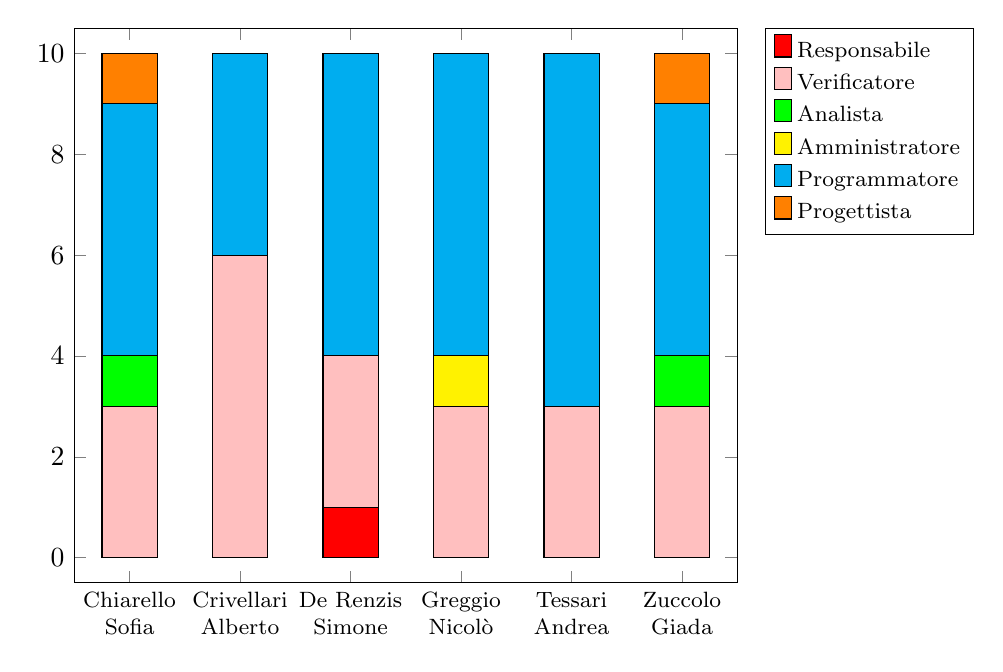
\begin{tikzpicture}
		\begin{axis}[
			enlarge y limits=0.05,
			enlarge x limits=0.10,
			ybar stacked,
			width=10cm,
			bar width=0.7cm,
			%every node near coord/.style={text width=3 cm},
			%nodes near coords,
			%every node near coord/.append style={color=black},
			%enlargelimits=0.25,
			legend style={font=\footnotesize,at={(1.2,1)},
				cells={anchor=west},
				anchor=north,legend columns=1},
			%ylabel={\#participants},
			symbolic x coords={Chiarello Sofia, Crivellari Alberto, De Renzis Simone, Greggio Nicolò, Tessari Andrea, Zuccolo Giada},
			xtick=data,
			x tick label style={font=\footnotesize,text width=1.7cm,align=center},
			]
			\addplot+[ybar,fill=red, draw=black] plot coordinates 
			%Responsabile
			{(Chiarello Sofia,0) 
				(Crivellari Alberto,0) 
				(De Renzis Simone,1) 
				(Greggio Nicolò,0) 
				(Tessari Andrea,0) 
				(Zuccolo Giada,0) };
			\addplot+[ybar,fill=pink, draw=black] plot coordinates 
			%Verificatore
			{(Chiarello Sofia,3) 
				(Crivellari Alberto,6) 
				(De Renzis Simone,3) 
				(Greggio Nicolò,3) 
				(Tessari Andrea,3) 
				(Zuccolo Giada,3) };
			\addplot+[ybar,fill=green, draw=black] plot coordinates 
			%Analista
			{(Chiarello Sofia,1) 
				(Crivellari Alberto,0) 
				(De Renzis Simone,0) 
				(Greggio Nicolò,0) 
				(Tessari Andrea,0) 
				(Zuccolo Giada,1) };
			\addplot+[ybar,fill=yellow, draw=black] plot coordinates
			%Amministratore
			{(Chiarello Sofia,0)
				(Crivellari Alberto,0) 
				(De Renzis Simone,0) 
				(Greggio Nicolò,1)
				(Tessari Andrea,0)
				(Zuccolo Giada,0) };
			\addplot+[ybar,fill=cyan, draw=black] plot coordinates 
			%Programmatore
			{(Chiarello Sofia,5) 
				(Crivellari Alberto,4) 
				(De Renzis Simone,6) 
				(Greggio Nicolò,6) 
				(Tessari Andrea,7) 
				(Zuccolo Giada,5) };
			\addplot+[ybar,fill=orange, draw=black] plot coordinates
			%Progettista
			{(Chiarello Sofia,1) 
				(Crivellari Alberto,0) 
				(De Renzis Simone,0)
				(Greggio Nicolò,0) 
				(Tessari Andrea,0) 
				(Zuccolo Giada,1) };
			\legend{Responsabile \\ Verificatore \\ Analista \\ Amministratore \\ Programmatore \\ Progettista \\}
		\end{axis}
	\end{tikzpicture}
	\caption[Istogramma distribuzione oraria Progettazione e Codifica dei Requisiti Desiderabili e Facoltativi]{Istogramma che visualizza la ripartizione delle ore nella fase\textsubscript{G} di Progettazione e Codifica dei Requisiti Desiderabili e Facoltativi} 
\end{figure}


\subsubsection{Prospetto economico}
Il costo derivante dalle ore impiegate dai componenti nella fase\textsubscript{G} di Progettazione e Codifica dei Requisiti Desiderabili e Facoltativi è descritto di seguito, calcolandone il totale.

\begin{table}[H]
	{\setlength{\parindent}{0cm}
		\begin{minipage}{.43\textwidth}
			\begin{tabular}{ccc}
				\rowcolorhead
				\headertitle{Ruolo} & \headertitle{Ore} & \headertitle{Costo(\euro{})}\\
				Responsabile & 1 & 30\\
				Verificatore & 21 & 315\\
				Analista & 2 & 50\\
				Amministratore & 1 & 20\\
				Programmatore & 33 & 495\\
				Progettista & 2 & 44\\
				\hline
				\textbf{Totale} & \textbf{60} & \textbf{954}\\
			\end{tabular}
		\end{minipage}% This must go next to `\end{minipage}`
		\begin{minipage}{.57\textwidth}
			\begin{tikzpicture}
				\pie [rotate = 270,
				sum = auto, 
				before number=\pgfsetfillopacity{0.0},
				%text = legend, 
				radius = 2.7,
				color = {red, pink, green, yellow, cyan, orange}]
				{
					30/Responsabile,
					315/Verificatore,
					50/Analista,
					20/Amministratore,
					495/Programmatore,
					44/Progettista
				}
			\end{tikzpicture} 
	\end{minipage} }
	\caption[Prospetto economico della fase\textsubscript{G} di Progettazione e Codifica dei Requisiti Desiderabili e Facoltativi]{Per ogni ruolo, il complessivo delle ore impiegate dai membri e il relativo ammontare in denaro. Il diagramma a torta visualizza la composizione dei costi nella fase\textsubscript{G} di Progettazione e Codifica dei Requisiti Desiderabili e Facoltativi}
\end{table}







\subsection{Validazione e Collaudo}

\subsubsection{Prospetto orario}
Di seguito viene illustrato l'utilizzo della risorsa\textsubscript{G} tempo (espresso in ore) dei vari componenti del gruppo nella fase\textsubscript{G} di Verifica e Collaudo:

\begin{table}[H]
	\begin{center}
		\begin{tabular}{c
				!{\color[HTML]{9b240a}\vrule width 1pt}
				cccccc
				!{\color[HTML]{9b240a}\vrule width 1pt}	
				c}
			\rowcolorhead
			\headertitle{Nome} & \headertitle{R} & \headertitle{V} & \headertitle{An} & \headertitle{Am} & \headertitle{Pr} & \headertitle{Pt} & \headertitle{Tot} \\
			
			Chiarello Sofia & 0 & 11 & 2 & 0 & 9 & 3 & 25\\
			Crivellari Alberto & 0 & 25 & 0 & 0 & 0 & 0 & 25\\
			De Renzis Simone & 2 & 12 & 0 & 0 & 8 & 3 & 25\\
			Greggio Nicolò & 0 & 14 & 0 & 2 & 6 & 3 & 25\\
			Tessari Andrea & 0 & 20 & 0 & 1 & 0 & 3 & 24\\
			Zuccolo Giada & 0 & 12 & 2 & 0 & 8 & 3 & 25\\
		\end{tabular}
		\caption[Occupazione oraria Verifica e Collaudo]{Per ogni componente, i ruoli ricoperti e la relativa occupazione oraria nella fase\textsubscript{G} di Verifica e Collaudo}
	\end{center}
\end{table}


\pgfplotsset{width=10cm,compat=1.17}
\begin{figure}[H]
	\centering
	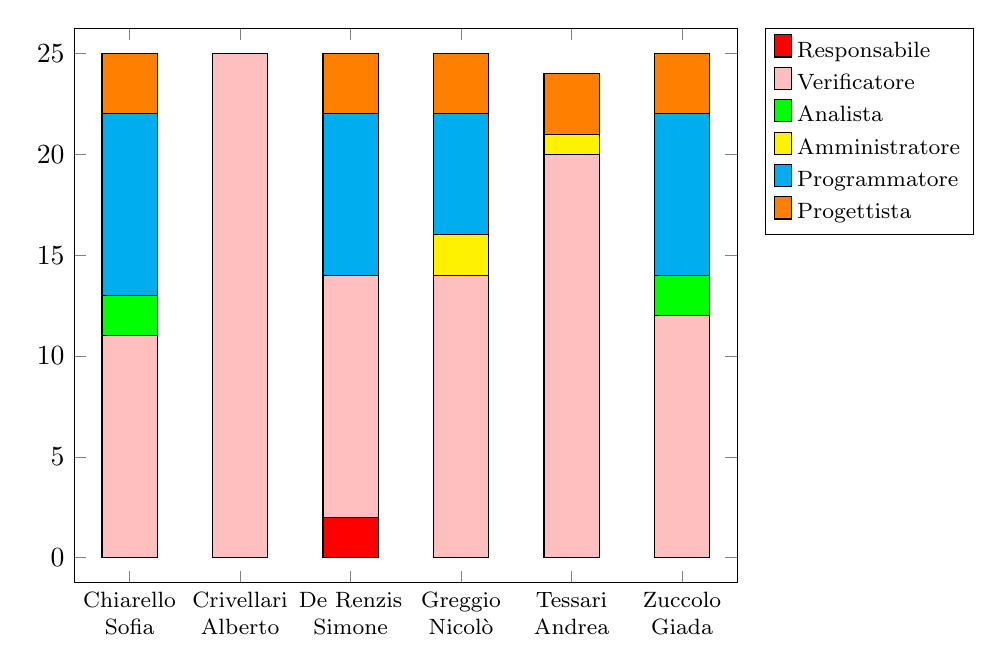
\begin{tikzpicture}
		\begin{axis}[
			enlarge y limits=0.05,
			enlarge x limits=0.10,
			ybar stacked,
			width=10cm,
			bar width=0.7cm,
			%every node near coord/.style={text width=3 cm},
			%nodes near coords,
			%every node near coord/.append style={color=black},
			%enlargelimits=0.25,
			legend style={font=\footnotesize,at={(1.2,1)},
				cells={anchor=west},
				anchor=north,legend columns=1},
			%ylabel={\#participants},
			symbolic x coords={Chiarello Sofia, Crivellari Alberto, De Renzis Simone, Greggio Nicolò, Tessari Andrea, Zuccolo Giada},
			xtick=data,
			x tick label style={font=\footnotesize,text width=1.7cm,align=center},
			]
			\addplot+[ybar,fill=red, draw=black] plot coordinates 
			%Responsabile
			{(Chiarello Sofia,0) 
				(Crivellari Alberto,0) 
				(De Renzis Simone,2) 
				(Greggio Nicolò,0) 
				(Tessari Andrea,0) 
				(Zuccolo Giada,0) };
			\addplot+[ybar,fill=pink, draw=black] plot coordinates 
			%Verificatore
			{(Chiarello Sofia,11) 
				(Crivellari Alberto,25) 
				(De Renzis Simone,12) 
				(Greggio Nicolò,14) 
				(Tessari Andrea,20) 
				(Zuccolo Giada,12) };
			\addplot+[ybar,fill=green, draw=black] plot coordinates 
			%Analista
			{(Chiarello Sofia,2) 
				(Crivellari Alberto,0) 
				(De Renzis Simone,0) 
				(Greggio Nicolò,0) 
				(Tessari Andrea,0) 
				(Zuccolo Giada,2) };
			\addplot+[ybar,fill=yellow, draw=black] plot coordinates
			%Amministratore
			{(Chiarello Sofia,0)
				(Crivellari Alberto,0) 
				(De Renzis Simone,0) 
				(Greggio Nicolò,2)
				(Tessari Andrea,1)
				(Zuccolo Giada,0) };
			\addplot+[ybar,fill=cyan, draw=black] plot coordinates 
			%Programmatore
			{(Chiarello Sofia,9) 
				(Crivellari Alberto,0) 
				(De Renzis Simone,8) 
				(Greggio Nicolò,6) 
				(Tessari Andrea,0) 
				(Zuccolo Giada,8) };
			\addplot+[ybar,fill=orange, draw=black] plot coordinates
			%Progettista
			{(Chiarello Sofia,3) 
				(Crivellari Alberto,0) 
				(De Renzis Simone,3)
				(Greggio Nicolò,3) 
				(Tessari Andrea,3) 
				(Zuccolo Giada,3) };
			\legend{Responsabile \\ Verificatore \\ Analista \\ Amministratore \\ Programmatore \\ Progettista \\}
		\end{axis}
	\end{tikzpicture}
	\caption[Istogramma distribuzione oraria Verifica e Collaudo]{Istogramma che visualizza la ripartizione delle ore nella fase\textsubscript{G} di Verifica e Collaudo} 
\end{figure}


\subsubsection{Prospetto economico}
Il costo derivante dalle ore impiegate dai componenti nella fase\textsubscript{G} di Verifica e Collaudo è descritto di seguito, calcolandone il totale.

\begin{table}[H]
	{\setlength{\parindent}{0cm}
		\begin{minipage}{.43\textwidth}
			\begin{tabular}{ccc}
				\rowcolorhead
				\headertitle{Ruolo} & \headertitle{Ore} & \headertitle{Costo(\euro{})}\\
				Responsabile & 2 & 60\\
				Verificatore & 94 & 1410\\
				Analista & 4 & 100\\
				Amministratore & 3 & 60\\
				Programmatore & 31 & 465\\
				Progettista & 15 & 330\\
				\hline
				\textbf{Totale} & \textbf{149} & \textbf{2425}\\
			\end{tabular}
		\end{minipage}% This must go next to `\end{minipage}`
		\begin{minipage}{.57\textwidth}
			\begin{tikzpicture}
				\pie [rotate = 270,
				sum = auto, 
				before number=\pgfsetfillopacity{0.0},
				%text = legend, 
				radius = 2.7,
				color = {red, pink, green, yellow, cyan, orange}]
				{
					60/Responsabile,
					1410/Verificatore,
					100/Analista,
					60/Amministratore,
					465/Programmatore,
					330/Progettista
				}
			\end{tikzpicture} 
	\end{minipage} }
	\caption[Prospetto economico della fase\textsubscript{G} di Verifica e Collaudo]{Per ogni ruolo, il complessivo delle ore impiegate dai membri e il relativo ammontare in denaro. Il diagramma a torta visualizza la composizione dei costi nella fase\textsubscript{G} di Verifica e Collaudo}
\end{table}



\newpage



\subsection{Riepilogo}

\subsubsection{Totale Ore}
Di seguito viene illustrato l'utilizzo totale della risorsa\textsubscript{G} tempo (espresso in ore) dei vari componenti del gruppo:

\begin{table}[H]
	\begin{center}
		\begin{tabular}{c
				!{\color[HTML]{9b240a}\vrule width 1pt}
				cccccc
				!{\color[HTML]{9b240a}\vrule width 1pt}	
				c}
			\rowcolorhead
			\headertitle{Nome} & \headertitle{R} & \headertitle{V} & \headertitle{An} & \headertitle{Am} & \headertitle{Pr} & \headertitle{Pt} & \headertitle{Tot} \\
			
			Chiarello Sofia & 3 & 39 & 32 & 1 & 44 & 25 & 144\\
			Crivellari Alberto & 3 & 77 & 9 & 3 & 29 & 23 & 144\\
			De Renzis Simone & 25 & 37 & 7 & 8 & 42 & 25 & 144\\
			Greggio Nicolò & 9 & 39 & 7 & 28 & 40 & 21 & 144\\
			Tessari Andrea & 13 & 47 & 9 & 13 & 32 & 30 & 144\\
			Zuccolo Giada & 3 & 39 & 32 & 3 & 44 & 23 & 144\\
		\end{tabular}
		\caption[Occupazione oraria totale]{Per ogni componente, i ruoli ricoperti e la relativa occupazione oraria per tutta la durata del lavoro}
	\end{center}
\end{table}


\pgfplotsset{width=10cm,compat=1.17}
\begin{figure}[H]
	\centering
	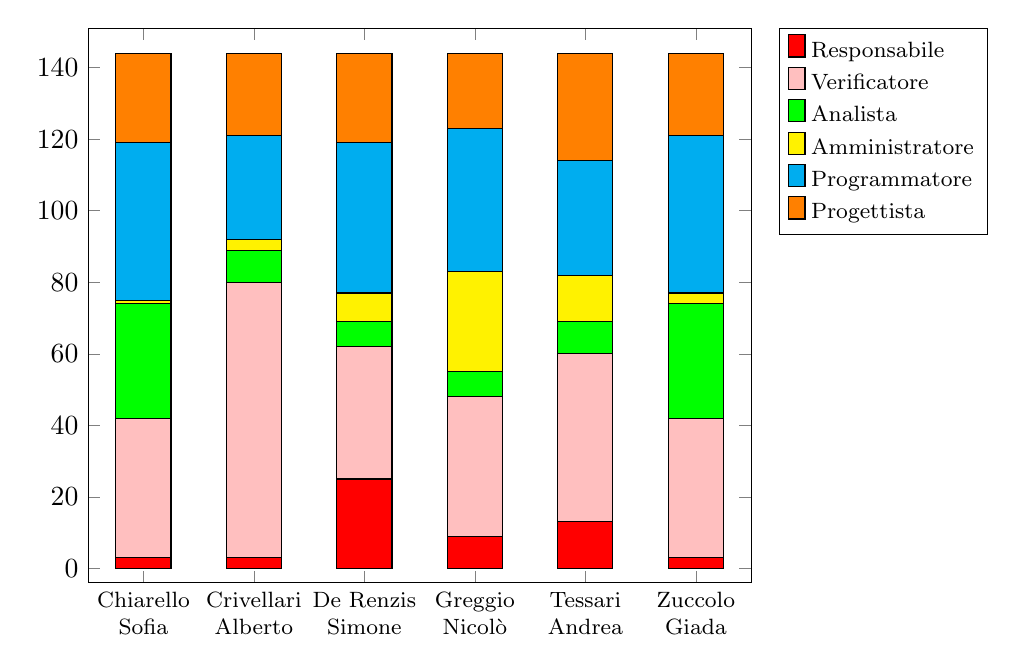
\begin{tikzpicture}
		\begin{axis}[
			enlarge y limits=0.05,
			enlarge x limits=0.10,
			ybar stacked,
			width=10cm,
			bar width=0.7cm,
			%every node near coord/.style={text width=3 cm},
			%nodes near coords,
			%every node near coord/.append style={color=black},
			%enlargelimits=0.25,
			legend style={font=\footnotesize,at={(1.2,1)},
				cells={anchor=west},
				anchor=north,legend columns=1},
			%ylabel={\#participants},
			symbolic x coords={Chiarello Sofia, Crivellari Alberto, De Renzis Simone, Greggio Nicolò, Tessari Andrea, Zuccolo Giada},
			xtick=data,
			x tick label style={font=\footnotesize,text width=1.7cm,align=center},
			]
			\addplot+[ybar,fill=red, draw=black] plot coordinates 
			%Responsabile
			{(Chiarello Sofia,3) 
				(Crivellari Alberto,3) 
				(De Renzis Simone,25) 
				(Greggio Nicolò,9) 
				(Tessari Andrea,13) 
				(Zuccolo Giada,3) };
			\addplot+[ybar,fill=pink, draw=black] plot coordinates 
			%Verificatore
			{(Chiarello Sofia,39) 
				(Crivellari Alberto,77) 
				(De Renzis Simone,37) 
				(Greggio Nicolò,39) 
				(Tessari Andrea,47) 
				(Zuccolo Giada,39) };
			\addplot+[ybar,fill=green, draw=black] plot coordinates 
			%Analista
			{(Chiarello Sofia,32) 
				(Crivellari Alberto,9) 
				(De Renzis Simone,7) 
				(Greggio Nicolò,7) 
				(Tessari Andrea,9) 
				(Zuccolo Giada,32) };
			\addplot+[ybar,fill=yellow, draw=black] plot coordinates
			%Amministratore
			{(Chiarello Sofia,1)
				(Crivellari Alberto,3) 
				(De Renzis Simone,8) 
				(Greggio Nicolò,28)
				(Tessari Andrea,13)
				(Zuccolo Giada,3) };
			\addplot+[ybar,fill=cyan, draw=black] plot coordinates 
			%Programmatore
			{(Chiarello Sofia,44) 
				(Crivellari Alberto,29) 
				(De Renzis Simone,42) 
				(Greggio Nicolò,40) 
				(Tessari Andrea,32) 
				(Zuccolo Giada,44) };
			\addplot+[ybar,fill=orange, draw=black] plot coordinates
			%Progettista
			{(Chiarello Sofia,25) 
				(Crivellari Alberto,23) 
				(De Renzis Simone,25)
				(Greggio Nicolò,21) 
				(Tessari Andrea,30) 
				(Zuccolo Giada,23) };
			\legend{Responsabile \\ Verificatore \\ Analista \\ Amministratore \\ Programmatore \\ Progettista \\}
		\end{axis}
	\end{tikzpicture}
	\caption[Istogramma distribuzione oraria totale]{Istogramma che visualizza la ripartizione delle ore per tutta la durata del lavoro} 
\end{figure}


\subsubsection{Prospetto economico}
Questa tabella mostra il costo totale per ogni ruolo all'interno del team. Viene evidenziato il totale.

\begin{table}[H]
	{\setlength{\parindent}{0cm}
		\begin{minipage}{.43\textwidth}
			\begin{tabular}{ccc}
				\rowcolorhead
				\headertitle{Ruolo} & \headertitle{Ore} & \headertitle{Costo(\euro{})}\\
				Responsabile & 56 & 1680\\
				Verificatore & 278 & 4170\\
				Analista & 96 & 2400\\
				Amministratore & 56 & 1120\\
				Programmatore & 231 & 3465\\
				Progettista & 147 & 3234\\
				\hline
				\textbf{Totale} & \textbf{864} & \textbf{16069}\\
			\end{tabular}
		\end{minipage}% This must go next to `\end{minipage}`
		\begin{minipage}{.57\textwidth}
			\begin{tikzpicture}
				\pie [rotate = 270,
				sum = auto, 
				before number=\pgfsetfillopacity{0.0},
				%text = legend, 
				radius = 2.7,
				color = {red, pink, green, yellow, cyan, orange}]
				{
					1680/Responsabile,
					4170/Verificatore,
					2400/Analista,
					1120/Amministratore,
					3465/Programmatore,
					3234/Progettista
				}
			\end{tikzpicture} 
	\end{minipage} }
	\caption[Prospetto economico complessivo]{Per ogni ruolo, il complessivo delle ore impiegate dai membri e il relativo ammontare in denaro. Il diagramma a torta visualizza la composizione dei costi complessivi}
\end{table}


\subsubsection{Ore rendicontate}


Questa tabella descrive il numero di ore rendicontate di ogni componente (sono cioè escluse le ore dedicate all'Avvio e all'Analisi dei Requisiti):

\begin{table}[H]
	\begin{center}
		\begin{tabular}{c
				!{\color[HTML]{9b240a}\vrule width 1pt}
				cccccc
				!{\color[HTML]{9b240a}\vrule width 1pt}	
				c}
			\rowcolorhead
			\headertitle{Nome} & \headertitle{R} & \headertitle{V} & \headertitle{An} & \headertitle{Am} & \headertitle{Pr} & \headertitle{Pt} & \headertitle{Tot} \\
			
			Chiarello Sofia & 1 & 31 & 9 & 0 & 44 & 25 & 110\\
			Crivellari Alberto & 1 & 57 & 0 & 1 & 29 & 23 & 111\\
			De Renzis Simone & 9 & 31 & 0 & 2 & 42 & 25 & 109\\
			Greggio Nicolò & 2 & 33 & 0 & 11 & 40 & 21 & 107\\
			Tessari Andrea & 3 & 40 & 0 & 5 & 32 & 30 & 110\\
			Zuccolo Giada & 1 & 31 & 9 & 2 & 44 & 23 & 110\\
		\end{tabular}
		\caption[Occupazione oraria totale rendicontata]{Per ogni componente, i ruoli ricoperti e la relativa occupazione oraria rendicontata totale}
	\end{center}
\end{table}


\pgfplotsset{width=10cm,compat=1.17}
\begin{figure}[H]
	\centering
	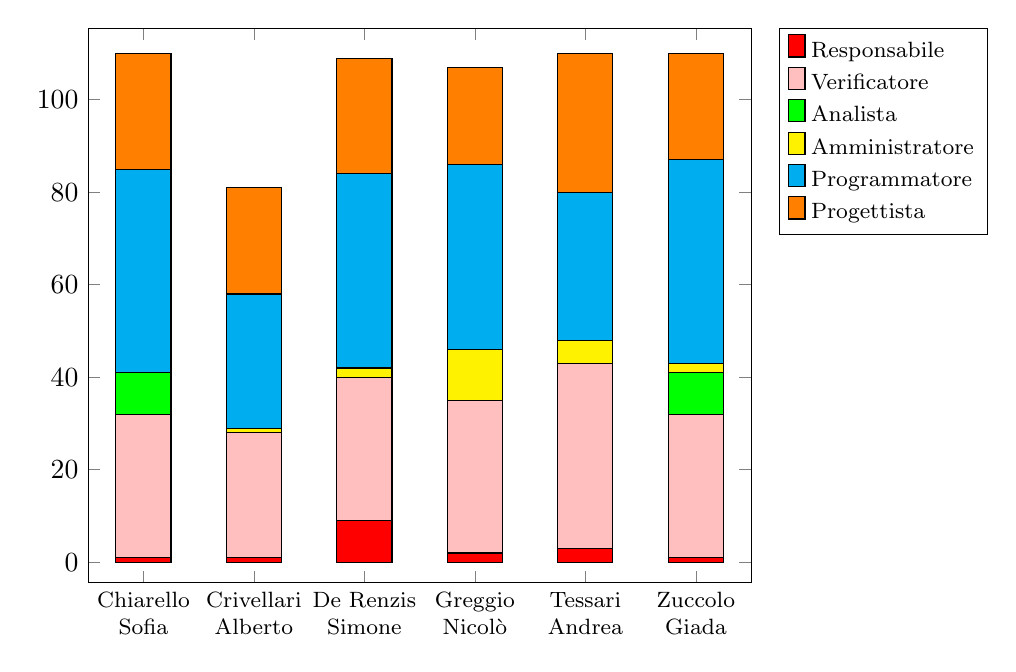
\begin{tikzpicture}
		\begin{axis}[
			enlarge y limits=0.05,
			enlarge x limits=0.10,
			ybar stacked,
			width=10cm,
			bar width=0.7cm,
			%every node near coord/.style={text width=3 cm},
			%nodes near coords,
			%every node near coord/.append style={color=black},
			%enlargelimits=0.25,
			legend style={font=\footnotesize,at={(1.2,1)},
				cells={anchor=west},
				anchor=north,legend columns=1},
			%ylabel={\#participants},
			symbolic x coords={Chiarello Sofia, Crivellari Alberto, De Renzis Simone, Greggio Nicolò, Tessari Andrea, Zuccolo Giada},
			xtick=data,
			x tick label style={font=\footnotesize,text width=1.7cm,align=center},
			]
			\addplot+[ybar,fill=red, draw=black] plot coordinates 
			%Responsabile
			{(Chiarello Sofia,1) 
				(Crivellari Alberto,1) 
				(De Renzis Simone,9) 
				(Greggio Nicolò,2) 
				(Tessari Andrea,3) 
				(Zuccolo Giada,1) };
			\addplot+[ybar,fill=pink, draw=black] plot coordinates 
			%Verificatore
			{(Chiarello Sofia,31) 
				(Crivellari Alberto,27) 
				(De Renzis Simone,31) 
				(Greggio Nicolò,33) 
				(Tessari Andrea,40) 
				(Zuccolo Giada,31) };
			\addplot+[ybar,fill=green, draw=black] plot coordinates 
			%Analista
			{(Chiarello Sofia,9) 
				(Crivellari Alberto,0) 
				(De Renzis Simone,0) 
				(Greggio Nicolò,0) 
				(Tessari Andrea,0) 
				(Zuccolo Giada,9) };
			\addplot+[ybar,fill=yellow, draw=black] plot coordinates
			%Amministratore
			{(Chiarello Sofia,0)
				(Crivellari Alberto,1) 
				(De Renzis Simone,2) 
				(Greggio Nicolò,11)
				(Tessari Andrea,5)
				(Zuccolo Giada,2) };
			\addplot+[ybar,fill=cyan, draw=black] plot coordinates 
			%Programmatore
			{(Chiarello Sofia,44) 
				(Crivellari Alberto,29) 
				(De Renzis Simone,42) 
				(Greggio Nicolò,40) 
				(Tessari Andrea,32) 
				(Zuccolo Giada,44) };
			\addplot+[ybar,fill=orange, draw=black] plot coordinates
			%Progettista
			{(Chiarello Sofia,25) 
				(Crivellari Alberto,23) 
				(De Renzis Simone,25)
				(Greggio Nicolò,21) 
				(Tessari Andrea,30) 
				(Zuccolo Giada,23) };
			\legend{Responsabile \\ Verificatore \\ Analista \\ Amministratore \\ Programmatore \\ Progettista \\}
		\end{axis}
	\end{tikzpicture}
	\caption[Istogramma distribuzione oraria rendicontata totale]{Istogramma che visualizza la ripartizione delle ore rendicontate per tutta la durata del lavoro} 
\end{figure}


\subsubsection{Prospetto economico ore rendicontate}
Questa tabella mostra il costo totale rendicontato per ogni ruolo all'interno del team. Viene evidenziato il totale.

\begin{table}[H]
	{\setlength{\parindent}{0cm}
		\begin{minipage}{.43\textwidth}
			\begin{tabular}{ccc}
				\rowcolorhead
				\headertitle{Ruolo} & \headertitle{Ore} & \headertitle{Costo(\euro{})}\\
				Responsabile & 17 & 510\\
				Verificatore & 223 & 3345\\
				Analista & 18 & 450\\
				Amministratore & 21 & 420\\
				Programmatore & 231 & 3465\\
				Progettista & 147 & 3234\\
				\hline
				\textbf{Totale} & \textbf{657} & \textbf{11424}\\
			\end{tabular}
		\end{minipage}% This must go next to `\end{minipage}`
		\begin{minipage}{.57\textwidth}
			\begin{tikzpicture}
				\pie [rotate = 270,
				sum = auto, 
				before number=\pgfsetfillopacity{0.0},
				%text = legend, 
				radius = 2.7,
				color = {red, pink, green, yellow, cyan, orange}]
				{
					510/Responsabile,
					3345/Verificatore,
					450/Analista,
					420/Amministratore,
					3465/Programmatore,
					3234/Progettista
				}
			\end{tikzpicture} 
	\end{minipage} }
	\caption[Prospetto economico complessivo delle ore rendicontate]{Per ogni ruolo, il complessivo delle ore rendicontate impiegate dai membri e il relativo ammontare in denaro. Il diagramma a torta visualizza la composizione dei costi complessivi rendicontati}
\end{table}


\subsection{Conclusione}
Il lavoro prevede costi per \textbf{11424 \euro{}}, tenendo conto solamente delle ore rendicontate.
